\subsection{Display}
\label{subsec:Hardware_Display}

Im Folgenden wird das Display geprüft. Da der Mikrocontroller den Programmfluss steuert, wird die einzige Aufgabe des Displays sein, dem Mikrocontroller zu melden, wenn ein Button gedrückt wurde. Es geht folglich darum, die UART-Schnittstelle zu prüfen.

\subsubsection{Test}\label{subsubsec:Display_Test}

In diesem Kapitel wird die Funktion des Displays verifiziert. Die Funktion wurde getestet, indem in der Nextion Software \textit{Nextion Editor} ein String über die UART-Schnittstelle ausgegeben und vom Oszilloskop abgebildet wurde. Der auszugebende String kann in der Software definiert und per Mikro-SD-Karte in den Programmspeicher des Displays geladen werden. Er wird versendet, sobald auf den ``Menu``-Knopf gedrückt wird, welcher in Abbildung \ref{fig:Hardware_Nextion_Display_0} zu erkennen ist.

\begin{figure}[h!]
	\centering
	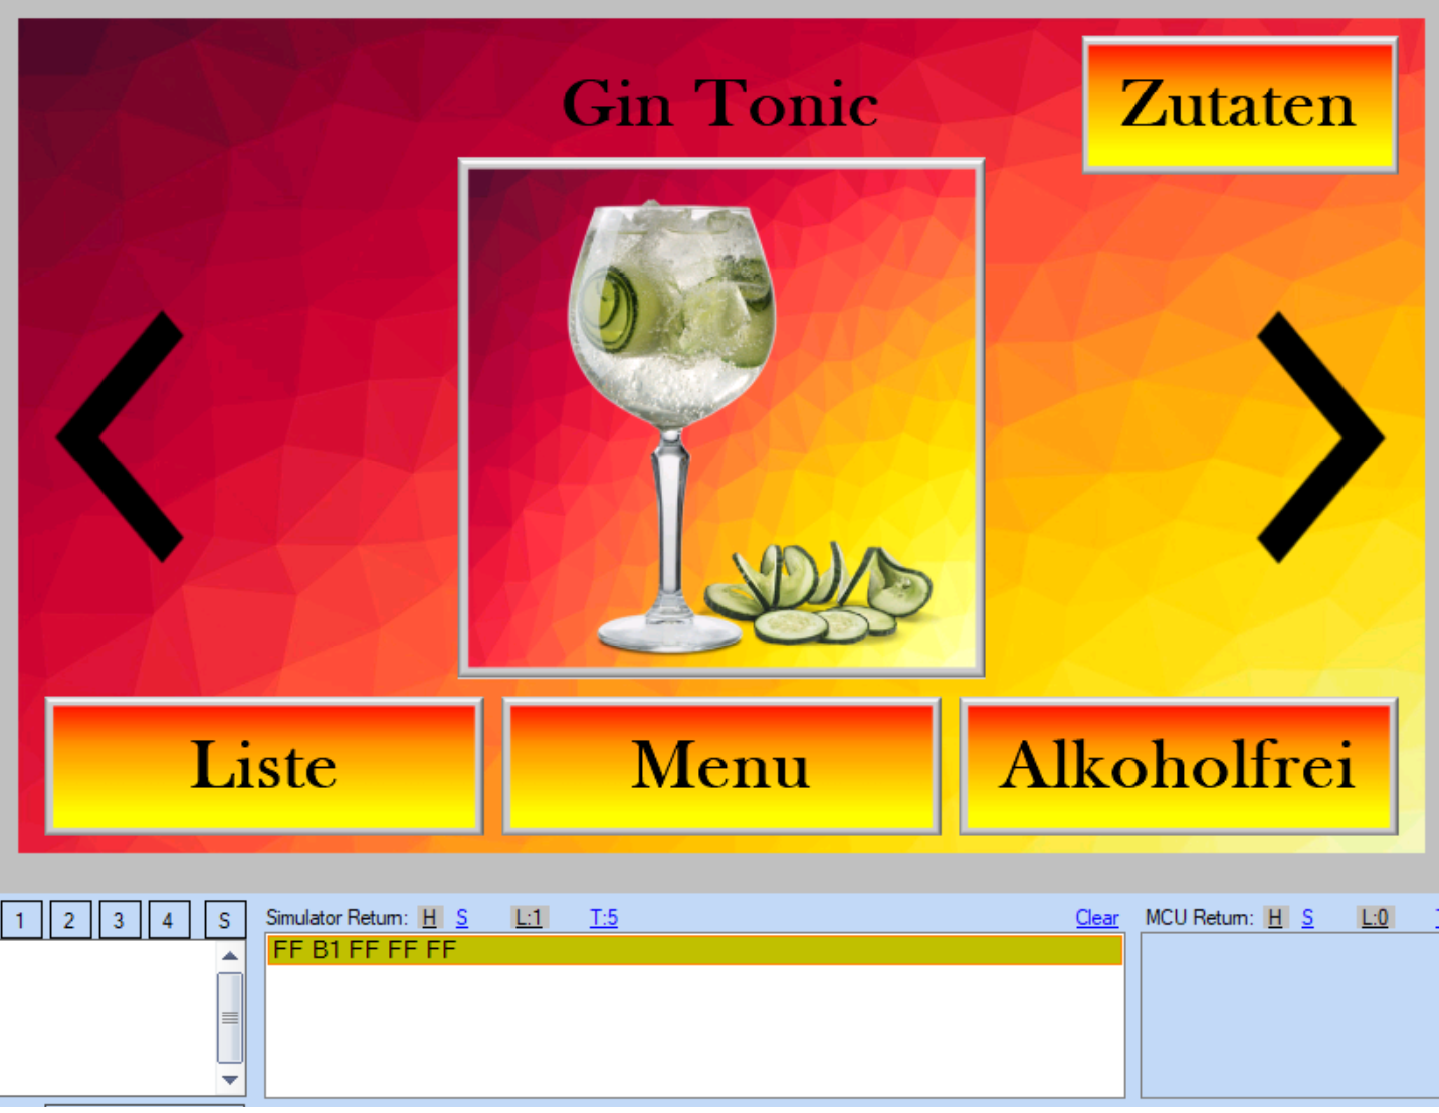
\includegraphics[width=0.7\textwidth]{graphics/Display_Hardware_Nextion_HMI.png}
	\caption{Nextion Software. Zu beachten: prinh-Funktion 0xFF 0xB1 0xFF 0xFF 0xFF.} 
	\label{fig:Hardware_Nextion_Display_0}
\end{figure}

\subsubsection{Erwartung}\label{subsubsec:Hardware_Display_Erwartung}

Der zu sendende String  wurde auf ``0xFF 0xB1 0xFF 0xFF 0xFF`` festgelegt und soll die ID des ``Menu``-Buttons wiederspiegeln, welcher sich auf Seite 0 befindet und Button 1 heisst. Das erste Zeichen (0xFF) gibt zu erkennen, auf welcher Seite wir uns befinden (eigentlich 0, doch es gab Probleme 0x00 zu interpretieren, weswegen entschieden wurde, anstelle von einem 0x00 ein 0xFF zu versenden). Die letzten drei Bytes (0xFF 0xFF 0xFF) geben das Ende der Übertragung zu erkennen. Wird der Button gedrückt, so wird erwartet, dass das Display die Seiten-ID gefolgt von der Button-ID und des Kommunikationsschlusses sendet.

\subsubsection{Ergebnis}\label{subsubsec:Hardware_Display_Ergebnis}
Die Abbildung \ref{fig:Hardware_Nextion_Display_0} zeigt, in welcher Folge die Daten an den Bus übergeben werden. Abbildung \ref{fig:Hardware_Nextion_Display_1} zeigt eine Abbildung des Oszilloskops, welches die Datenübertragung festhält. 

\begin{figure}[h!]
	\centering
	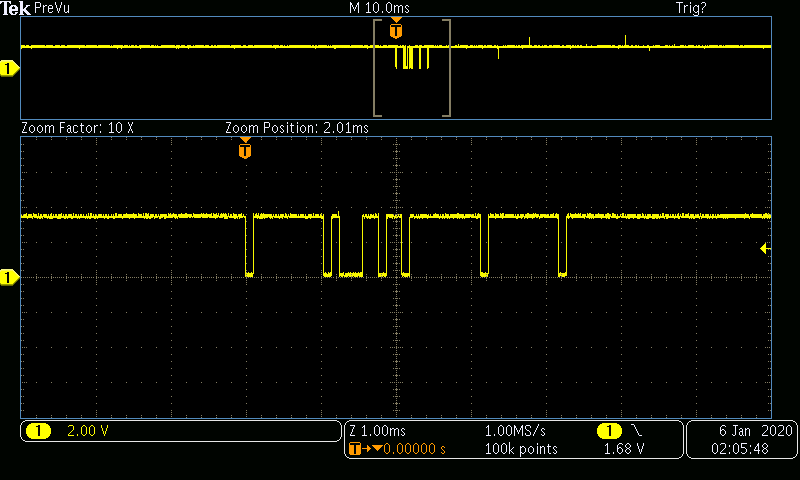
\includegraphics[width=0.8\textwidth]{graphics/Messung_UART_Nextion_Display.png}
	\caption{Messung gesendeter Daten des Displays. Zu beachten: 0xFF 0xB1 0xFF 0xFF 0xFF.} 
	\label{fig:Hardware_Nextion_Display_1}
\end{figure}

Wie zu erkennen ist, stimmt die Datenfolge, welche vom Display an den Bus weitergegeben wird, die Funktion ist somit bestätigt.

Wichtig ist die Reihenfolge der Bits, wie zu erkennen ist, findet die Übertragung mit dem LSB-first statt, entgegen der SPI-Schnitstelle, welche mit dem MSB-first kommuniziert.